\documentclass[a4paper, 50pt, twoside]{article}
\usepackage[italian]{babel}
\usepackage[a4paper, top=2cm, bottom=2cm, left=3cm, right=3cm]{geometry}
\usepackage{graphicx}
\graphicspath{{immagini/}}
\usepackage{chngcntr}
\counterwithin{figure}{section}
\usepackage{braket}
\usepackage{amsmath}
\usepackage{fancyhdr}
\usepackage{xcolor}
\pagestyle{fancy}
\lfoot{EasyVersity}

\begin{document}


\title{Relazione progetto Programmazione mobile}
\date{Settembre, 2019}
\author{Tomassini Danilo, Simone Cappella, Luca Mannini \\ Ingegneria Informatica e dell'Automazione}
\maketitle
\vspace*{\fill}
\vspace*{\fill}

\newpage
\tableofcontents{}

\newpage
\section{Obbiettivi}
EasyVersity rappresenta uno strumento di supporto per lo studente.

Permette di gestire:
\begin{itemize}
\item \textbf{Orario:} salva l'orario delle lezioni nella tua applicazione per consultarlo quando vuoi.
\item \textbf{Archivio appunti locale:} da la possibilità di salvare appunti raggruppandoli per materia, indicando titolo e data si può contestualizzare al meglio l'appunto in questione.
\item \textbf{Condivisione appunti:} rende possibile la condivisione ed il download degli appunti.
\item \textbf{Impostazioni:} da qui si possono cambiare informazioni come username e password, eprendere visione di info "about us".
\end{itemize}

\section{Funzionalità}
All'avvio dell'applicazione va effettuato il login o la registrazione.
\begin{figure}[!h]
	\centering
	{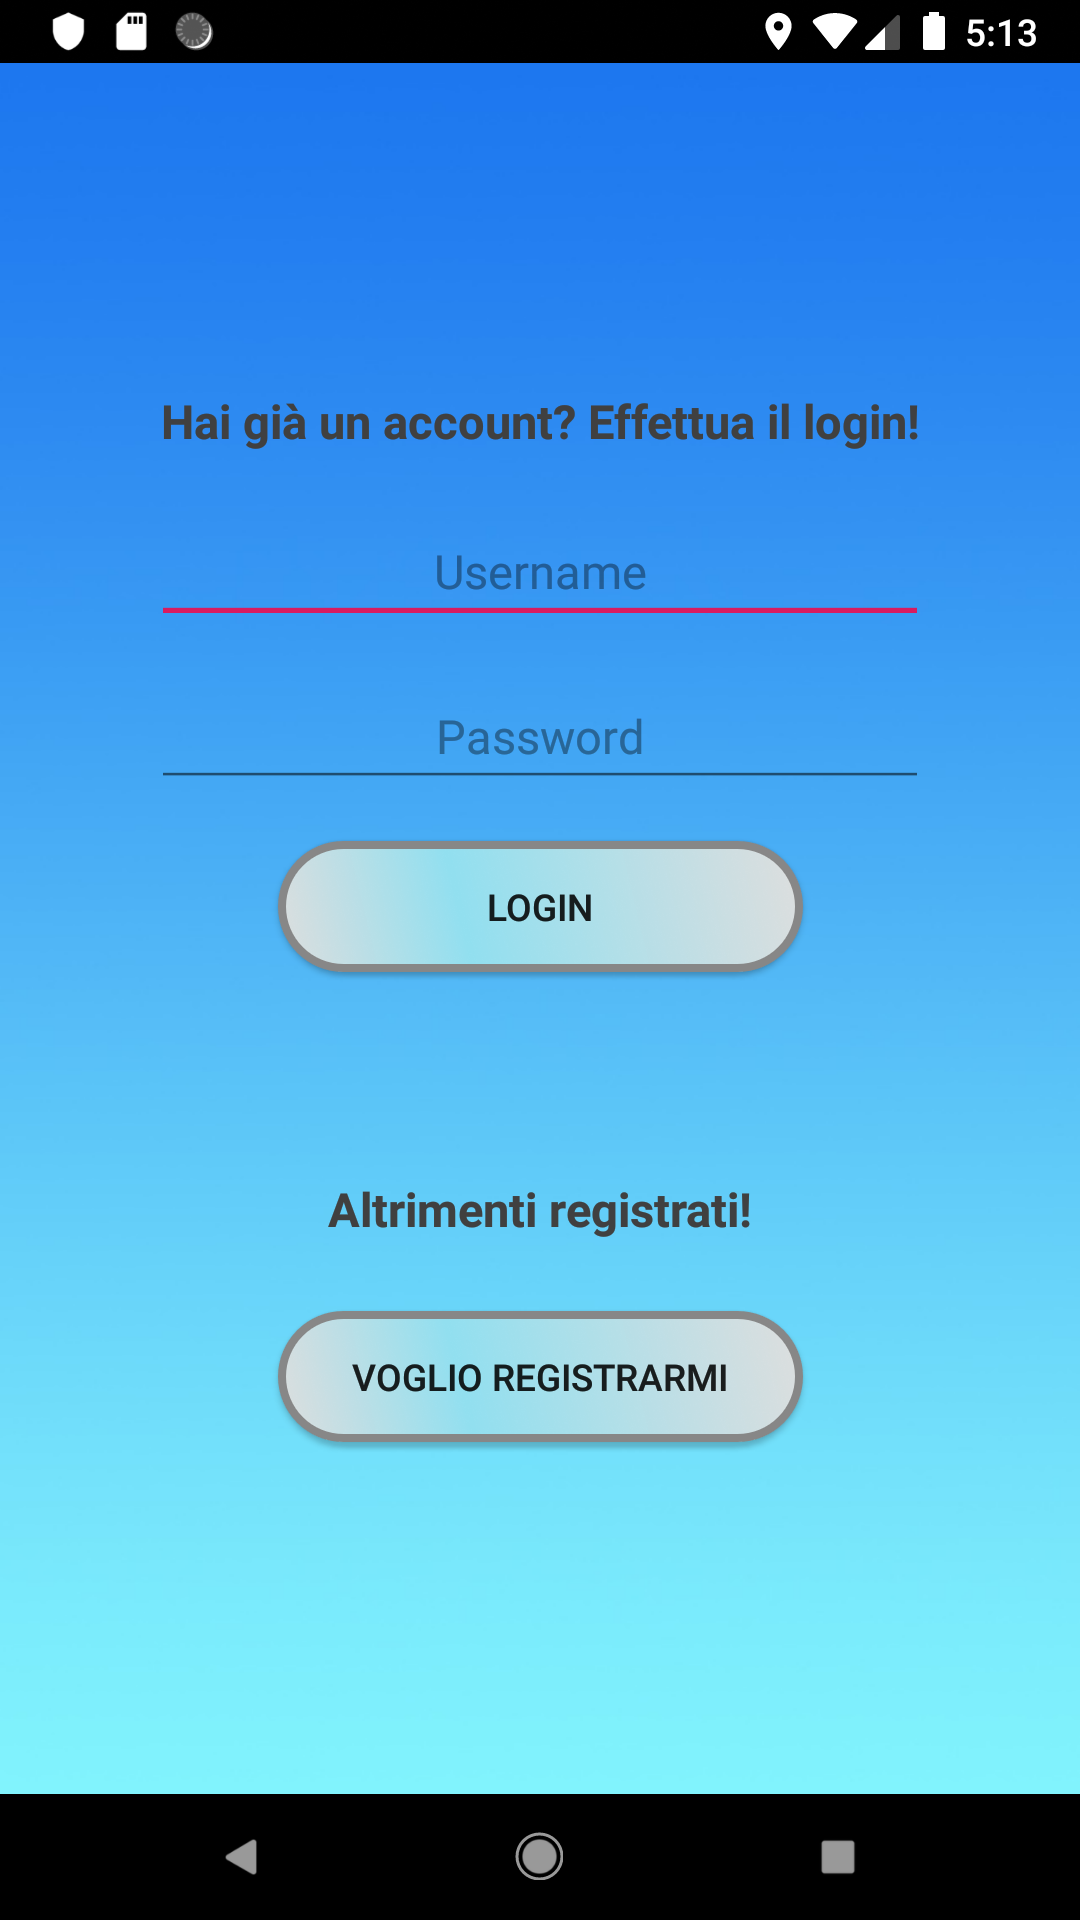
\includegraphics[width=.30\textwidth]{login}} \quad
	{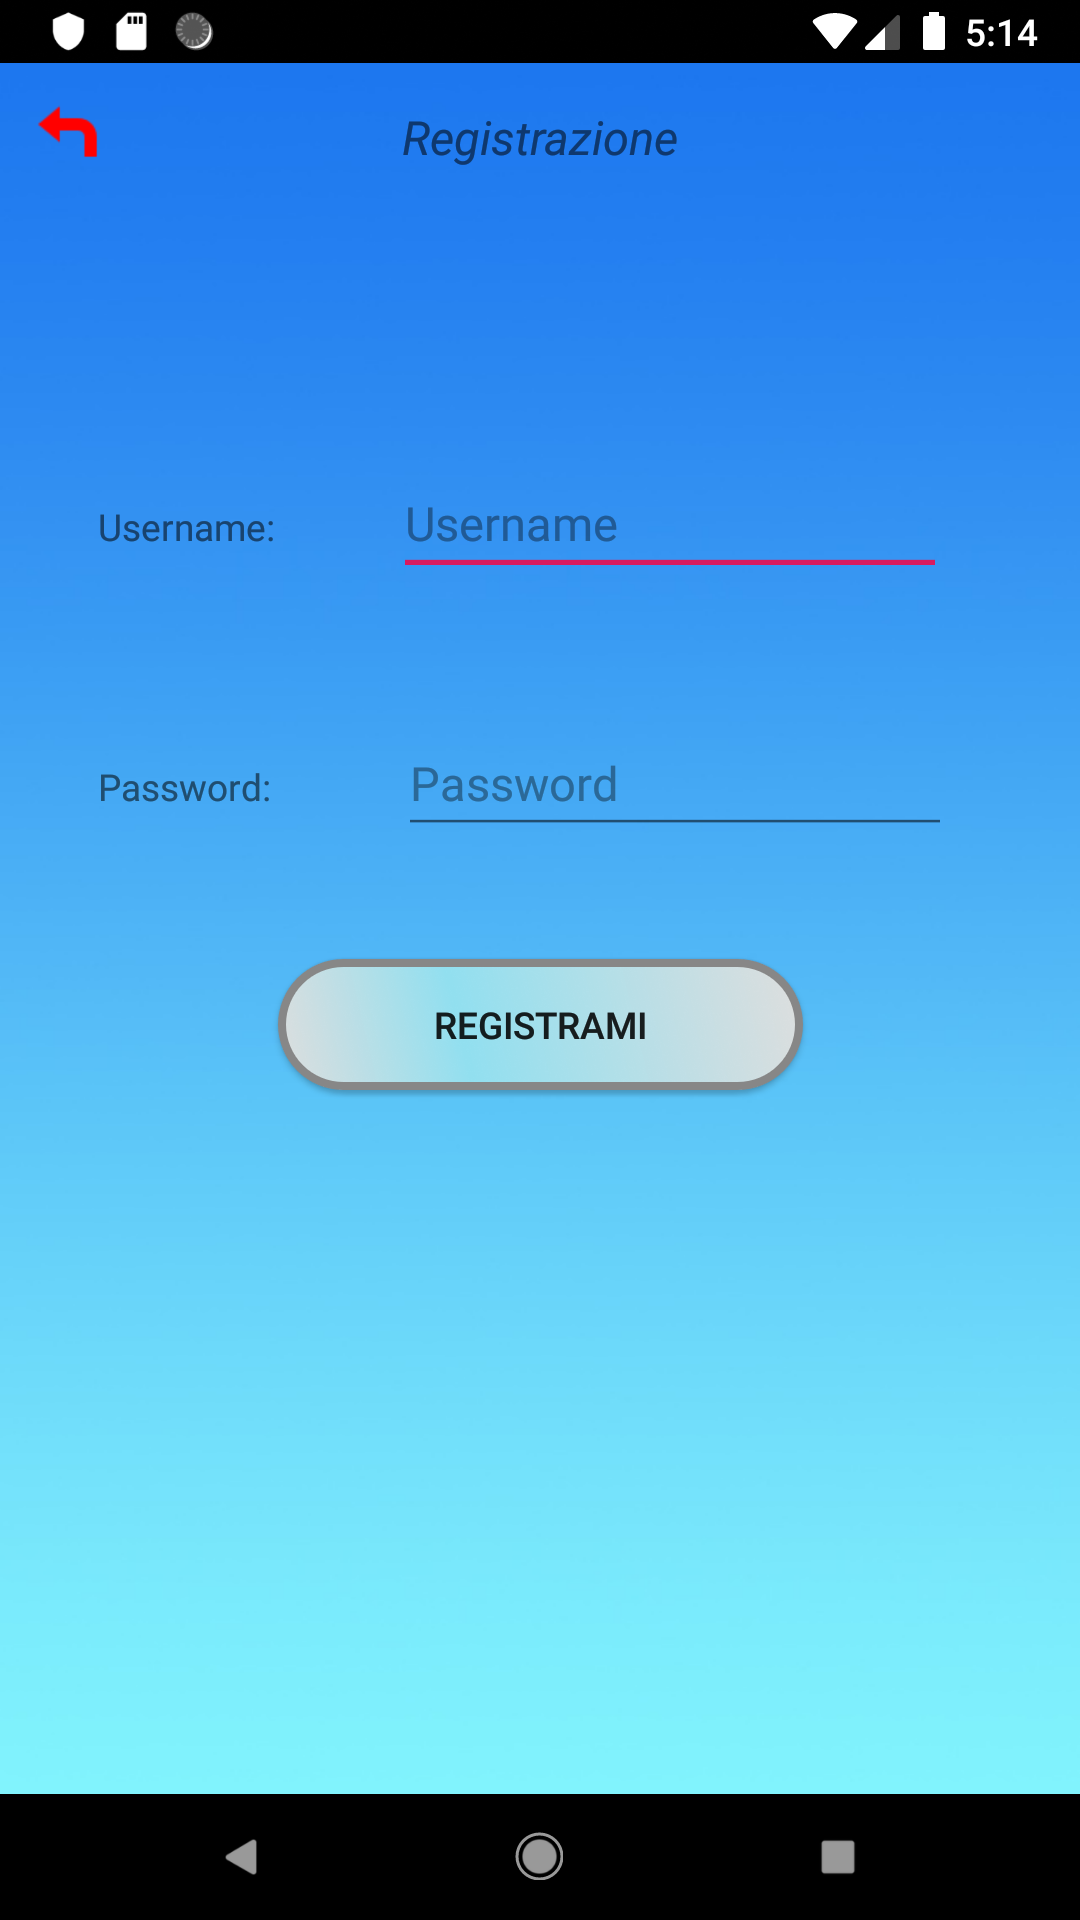
\includegraphics[width=.30\textwidth]{registrazione}}
	\caption{\small Schermata Login e Registrazione.}
\end{figure}

Una volta effettuato il login si può accedere al menù principale che prevede 4 scelte:
\begin{itemize}
\item \textbf{Orario.}
\item \textbf{I miei appunti.}
\item \textbf{Appunti condivisi.}
\item \textbf{Impostazioni.}
\end{itemize}

\begin{figure}[!h]
	\centering
	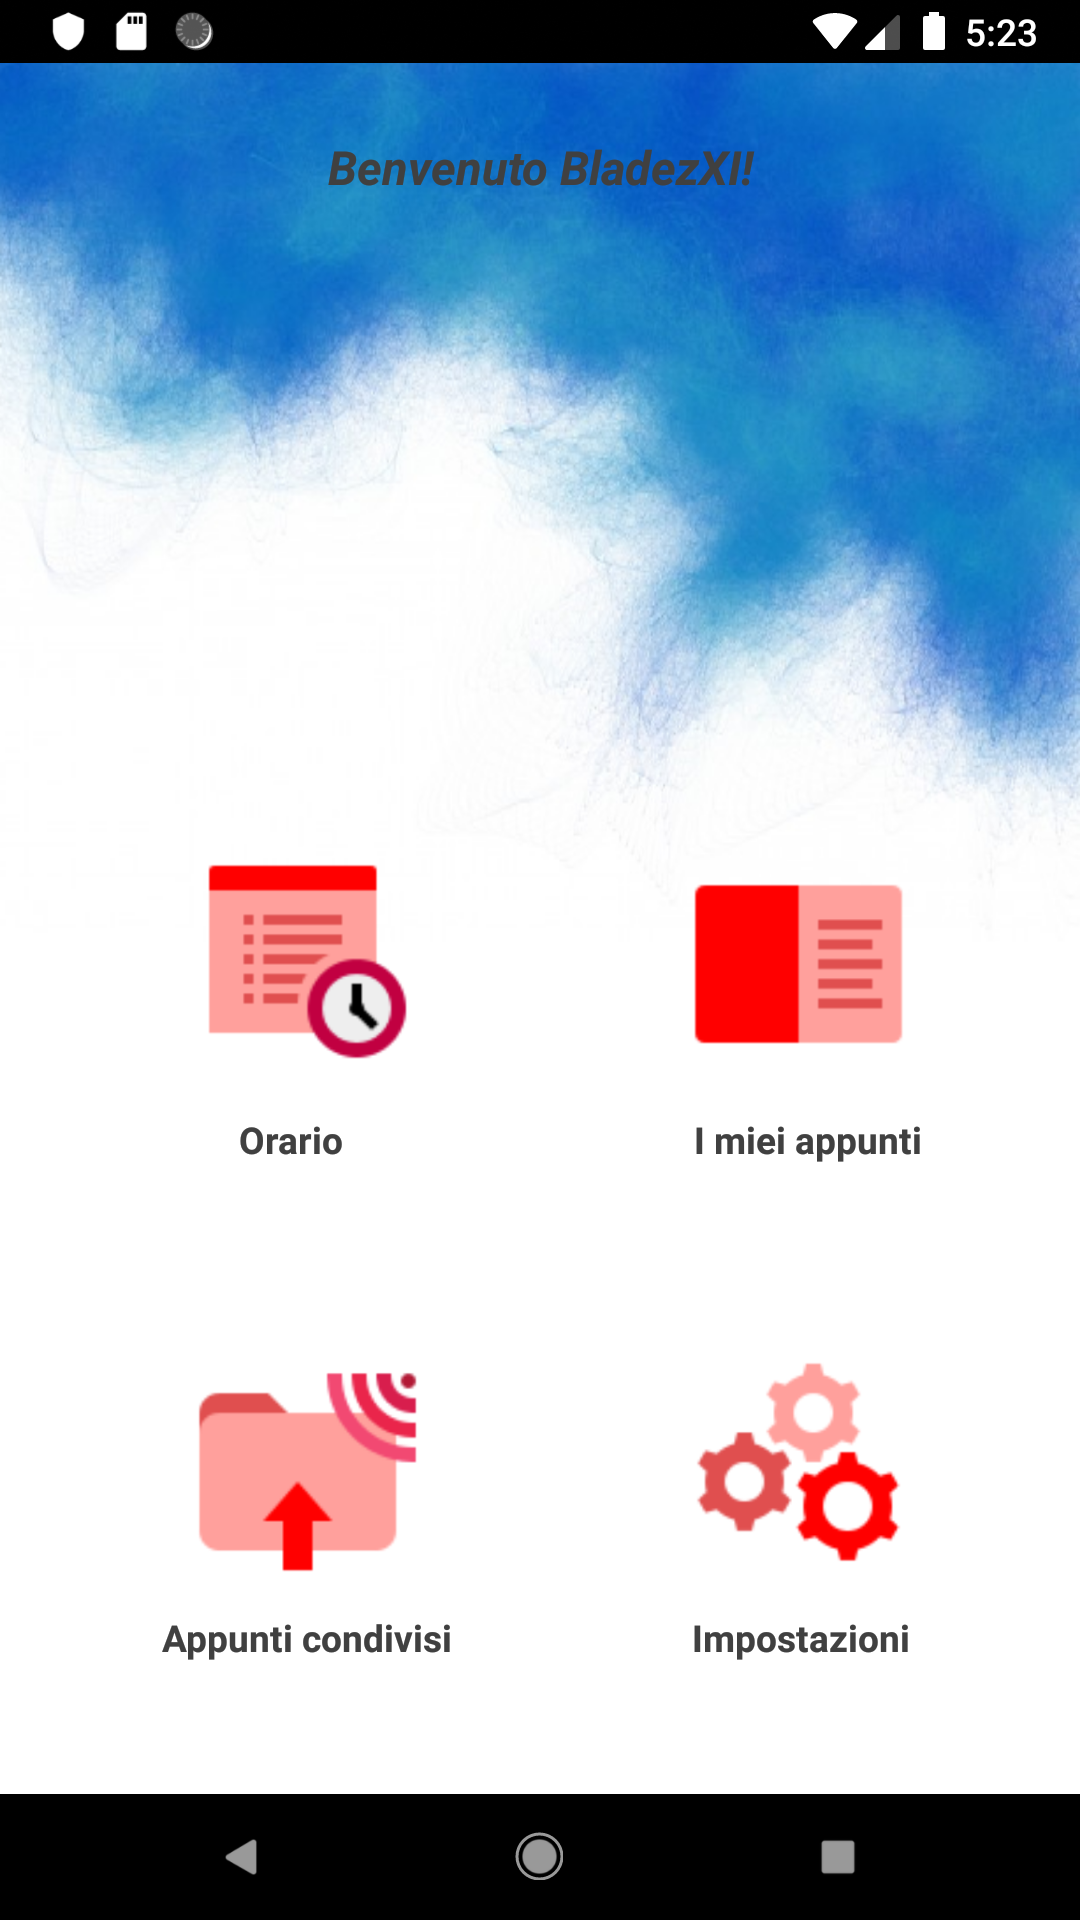
\includegraphics[width=.30\textwidth]{menu}
	\caption{\small Schermata di scelta principale.}
\end{figure}
\newpage
\subsection{Orario}
Aperto l'orario ci si trova di fronte alla tabella relativa al giorno corrente; con la bottom navbar si può scegliere il giorno su cui andare ad agire.
Premendo nel campo \textbf{materia}, relativo all'ora di interesse si può inserire la materia in tabella, si accede, infatti, ad una lista predefinita di materie (questa può essere estesa scegliendo di inserirne una manualmente con il bottone "altro"). Scelta la materia viene visualizzata una finestra di dialogo che permette di inserire l'aula in cui si svolgerà la lezione e la durata della stessa.
\begin{figure}[!h]
	\centering
	{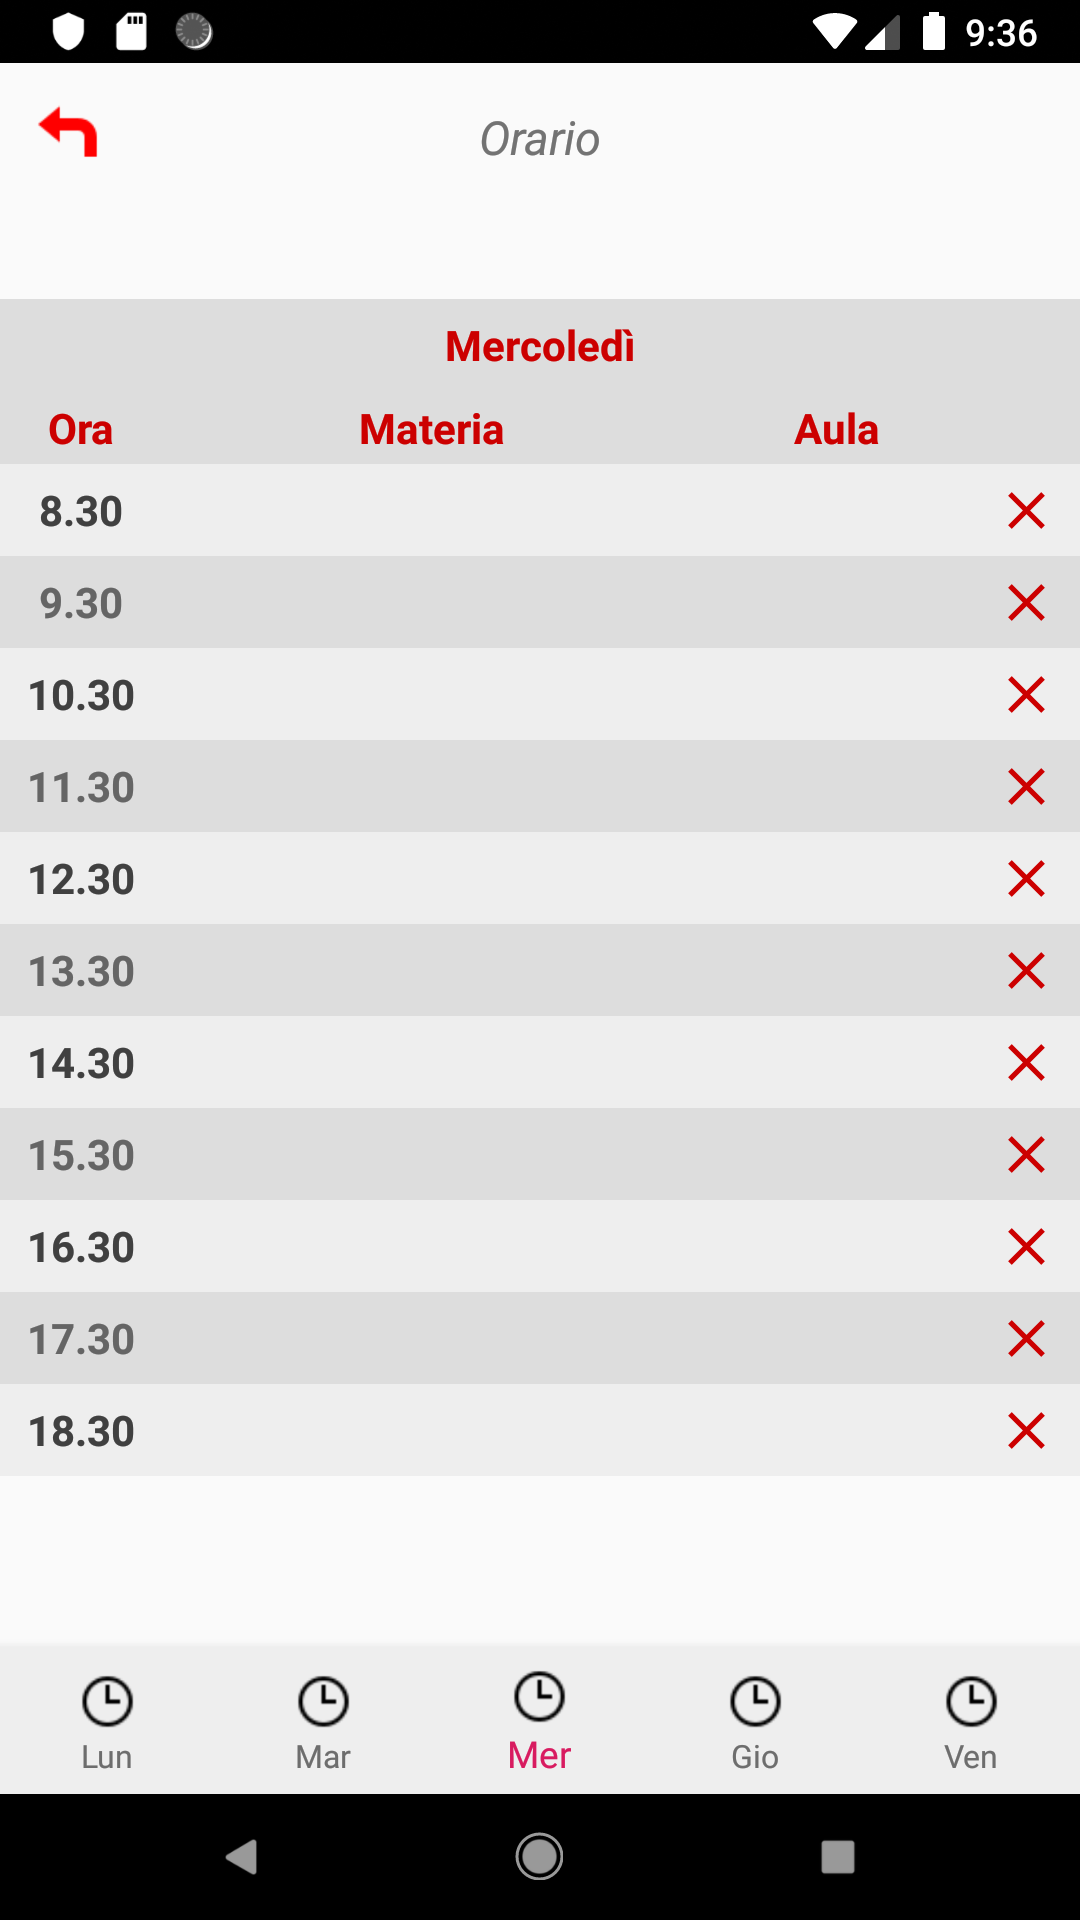
\includegraphics[width=.30\textwidth]{orario}} \quad
	{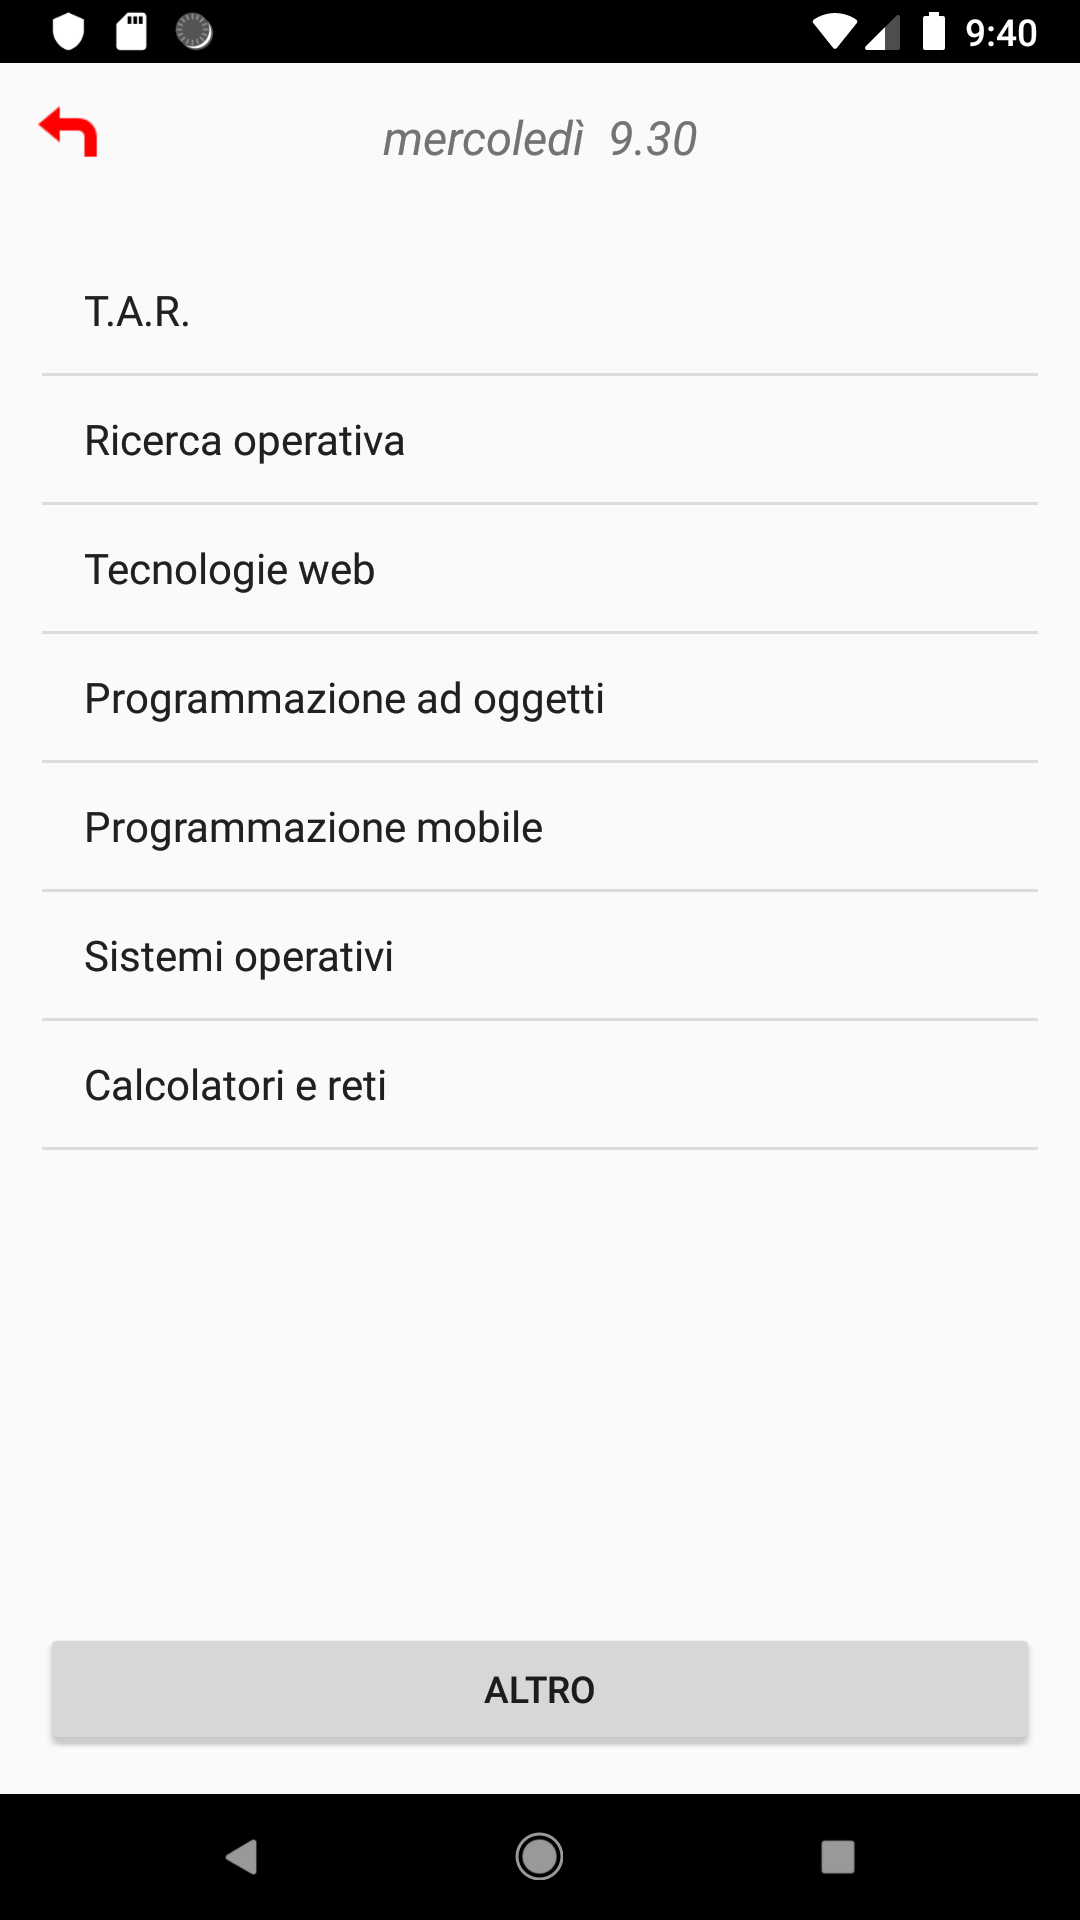
\includegraphics[width=.30\textwidth]{orario_scelta_materia}}\quad
	{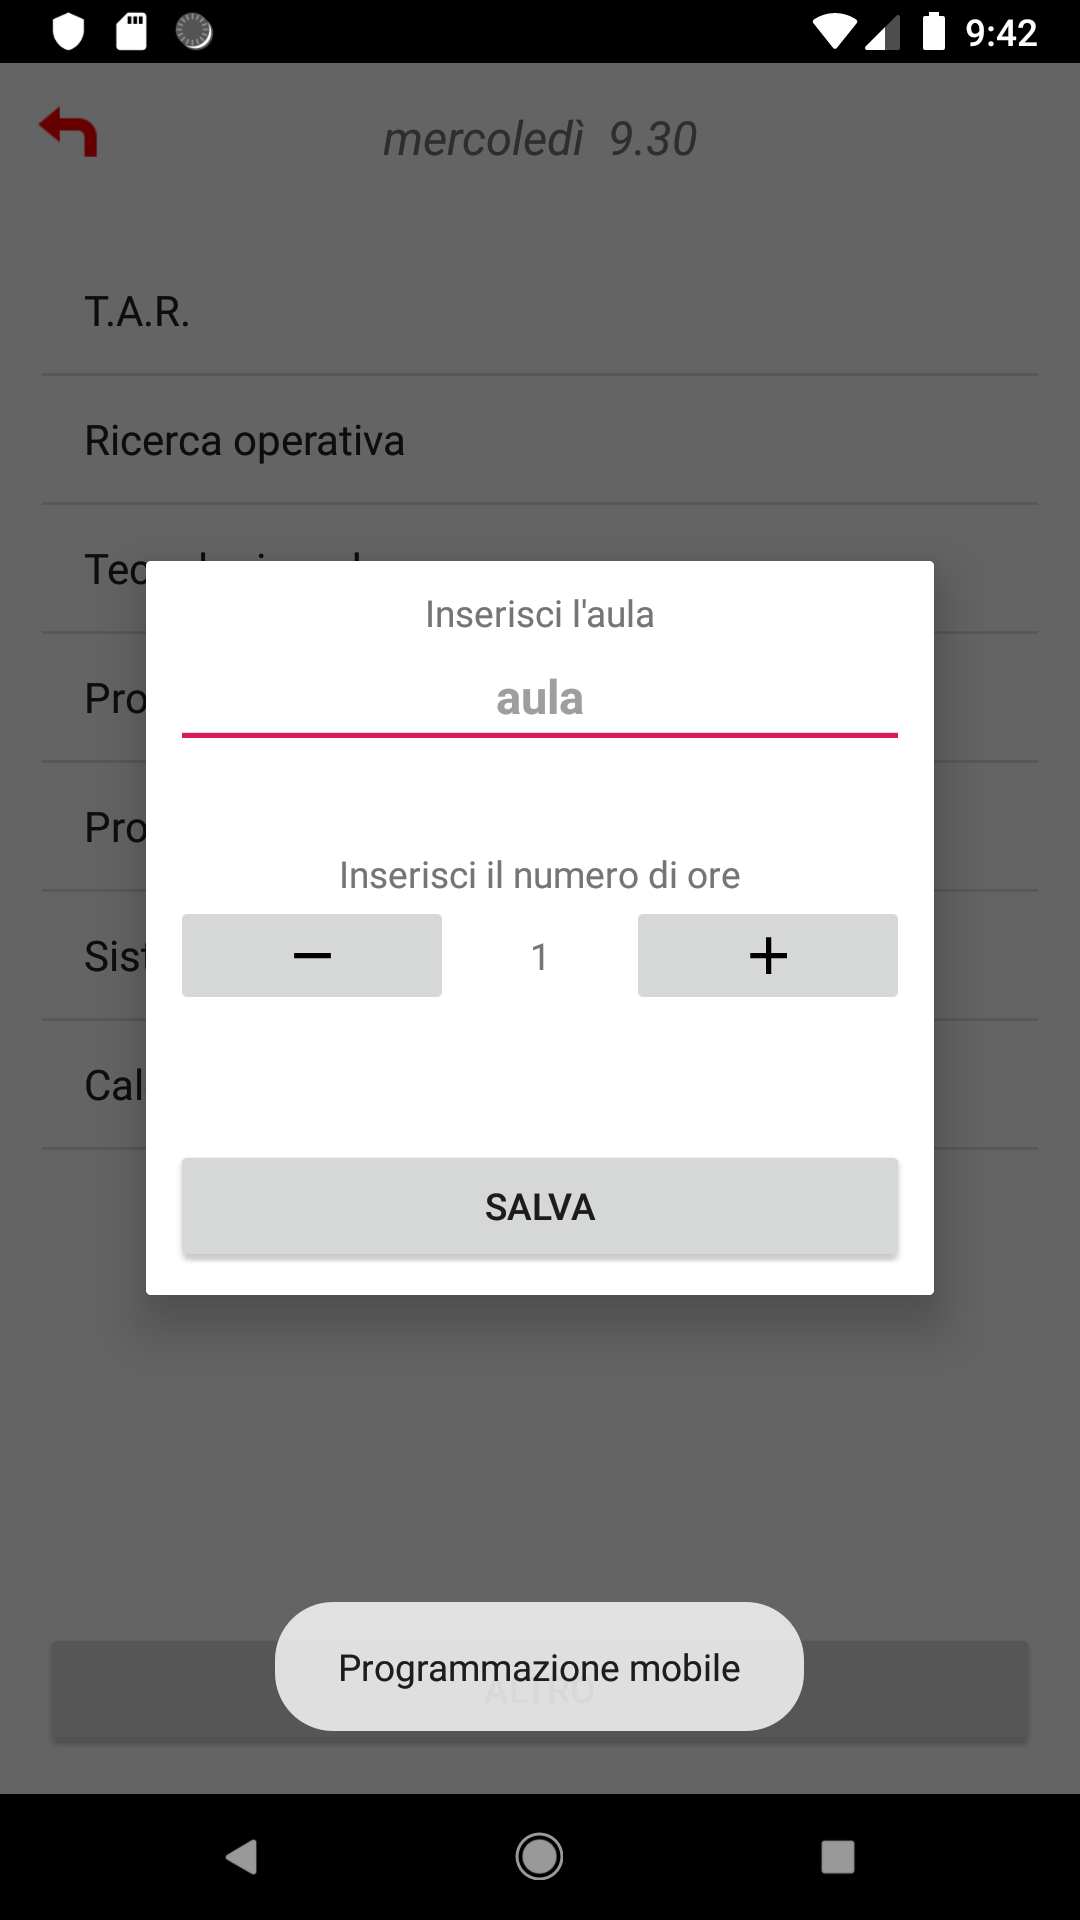
\includegraphics[width=.30\textwidth]{orario_inserimento}}
	\caption{\small Orario.}
\end{figure}

Salvata la materia nell'orario questa viene salvata nel database e inserita in una lista nella sezione \textbf{i miei appunti}.

\subsection{I miei appunti}
In questa sezione abbiamo accesso alla lista di tutte le materie salvate 




























































\end{document}